% Options for packages loaded elsewhere
\PassOptionsToPackage{unicode}{hyperref}
\PassOptionsToPackage{hyphens}{url}
%
\documentclass[
]{article}
\usepackage{amsmath,amssymb}
\usepackage{iftex}
\ifPDFTeX
  \usepackage[T1]{fontenc}
  \usepackage[utf8]{inputenc}
  \usepackage{textcomp} % provide euro and other symbols
\else % if luatex or xetex
  \usepackage{unicode-math} % this also loads fontspec
  \defaultfontfeatures{Scale=MatchLowercase}
  \defaultfontfeatures[\rmfamily]{Ligatures=TeX,Scale=1}
\fi
\usepackage{lmodern}
\ifPDFTeX\else
  % xetex/luatex font selection
\fi
% Use upquote if available, for straight quotes in verbatim environments
\IfFileExists{upquote.sty}{\usepackage{upquote}}{}
\IfFileExists{microtype.sty}{% use microtype if available
  \usepackage[]{microtype}
  \UseMicrotypeSet[protrusion]{basicmath} % disable protrusion for tt fonts
}{}
\makeatletter
\@ifundefined{KOMAClassName}{% if non-KOMA class
  \IfFileExists{parskip.sty}{%
    \usepackage{parskip}
  }{% else
    \setlength{\parindent}{0pt}
    \setlength{\parskip}{6pt plus 2pt minus 1pt}}
}{% if KOMA class
  \KOMAoptions{parskip=half}}
\makeatother
\usepackage{xcolor}
\usepackage[margin=1in]{geometry}
\usepackage{color}
\usepackage{fancyvrb}
\newcommand{\VerbBar}{|}
\newcommand{\VERB}{\Verb[commandchars=\\\{\}]}
\DefineVerbatimEnvironment{Highlighting}{Verbatim}{commandchars=\\\{\}}
% Add ',fontsize=\small' for more characters per line
\usepackage{framed}
\definecolor{shadecolor}{RGB}{248,248,248}
\newenvironment{Shaded}{\begin{snugshade}}{\end{snugshade}}
\newcommand{\AlertTok}[1]{\textcolor[rgb]{0.94,0.16,0.16}{#1}}
\newcommand{\AnnotationTok}[1]{\textcolor[rgb]{0.56,0.35,0.01}{\textbf{\textit{#1}}}}
\newcommand{\AttributeTok}[1]{\textcolor[rgb]{0.13,0.29,0.53}{#1}}
\newcommand{\BaseNTok}[1]{\textcolor[rgb]{0.00,0.00,0.81}{#1}}
\newcommand{\BuiltInTok}[1]{#1}
\newcommand{\CharTok}[1]{\textcolor[rgb]{0.31,0.60,0.02}{#1}}
\newcommand{\CommentTok}[1]{\textcolor[rgb]{0.56,0.35,0.01}{\textit{#1}}}
\newcommand{\CommentVarTok}[1]{\textcolor[rgb]{0.56,0.35,0.01}{\textbf{\textit{#1}}}}
\newcommand{\ConstantTok}[1]{\textcolor[rgb]{0.56,0.35,0.01}{#1}}
\newcommand{\ControlFlowTok}[1]{\textcolor[rgb]{0.13,0.29,0.53}{\textbf{#1}}}
\newcommand{\DataTypeTok}[1]{\textcolor[rgb]{0.13,0.29,0.53}{#1}}
\newcommand{\DecValTok}[1]{\textcolor[rgb]{0.00,0.00,0.81}{#1}}
\newcommand{\DocumentationTok}[1]{\textcolor[rgb]{0.56,0.35,0.01}{\textbf{\textit{#1}}}}
\newcommand{\ErrorTok}[1]{\textcolor[rgb]{0.64,0.00,0.00}{\textbf{#1}}}
\newcommand{\ExtensionTok}[1]{#1}
\newcommand{\FloatTok}[1]{\textcolor[rgb]{0.00,0.00,0.81}{#1}}
\newcommand{\FunctionTok}[1]{\textcolor[rgb]{0.13,0.29,0.53}{\textbf{#1}}}
\newcommand{\ImportTok}[1]{#1}
\newcommand{\InformationTok}[1]{\textcolor[rgb]{0.56,0.35,0.01}{\textbf{\textit{#1}}}}
\newcommand{\KeywordTok}[1]{\textcolor[rgb]{0.13,0.29,0.53}{\textbf{#1}}}
\newcommand{\NormalTok}[1]{#1}
\newcommand{\OperatorTok}[1]{\textcolor[rgb]{0.81,0.36,0.00}{\textbf{#1}}}
\newcommand{\OtherTok}[1]{\textcolor[rgb]{0.56,0.35,0.01}{#1}}
\newcommand{\PreprocessorTok}[1]{\textcolor[rgb]{0.56,0.35,0.01}{\textit{#1}}}
\newcommand{\RegionMarkerTok}[1]{#1}
\newcommand{\SpecialCharTok}[1]{\textcolor[rgb]{0.81,0.36,0.00}{\textbf{#1}}}
\newcommand{\SpecialStringTok}[1]{\textcolor[rgb]{0.31,0.60,0.02}{#1}}
\newcommand{\StringTok}[1]{\textcolor[rgb]{0.31,0.60,0.02}{#1}}
\newcommand{\VariableTok}[1]{\textcolor[rgb]{0.00,0.00,0.00}{#1}}
\newcommand{\VerbatimStringTok}[1]{\textcolor[rgb]{0.31,0.60,0.02}{#1}}
\newcommand{\WarningTok}[1]{\textcolor[rgb]{0.56,0.35,0.01}{\textbf{\textit{#1}}}}
\usepackage{longtable,booktabs,array}
\usepackage{calc} % for calculating minipage widths
% Correct order of tables after \paragraph or \subparagraph
\usepackage{etoolbox}
\makeatletter
\patchcmd\longtable{\par}{\if@noskipsec\mbox{}\fi\par}{}{}
\makeatother
% Allow footnotes in longtable head/foot
\IfFileExists{footnotehyper.sty}{\usepackage{footnotehyper}}{\usepackage{footnote}}
\makesavenoteenv{longtable}
\usepackage{graphicx}
\makeatletter
\def\maxwidth{\ifdim\Gin@nat@width>\linewidth\linewidth\else\Gin@nat@width\fi}
\def\maxheight{\ifdim\Gin@nat@height>\textheight\textheight\else\Gin@nat@height\fi}
\makeatother
% Scale images if necessary, so that they will not overflow the page
% margins by default, and it is still possible to overwrite the defaults
% using explicit options in \includegraphics[width, height, ...]{}
\setkeys{Gin}{width=\maxwidth,height=\maxheight,keepaspectratio}
% Set default figure placement to htbp
\makeatletter
\def\fps@figure{htbp}
\makeatother
\setlength{\emergencystretch}{3em} % prevent overfull lines
\providecommand{\tightlist}{%
  \setlength{\itemsep}{0pt}\setlength{\parskip}{0pt}}
\setcounter{secnumdepth}{-\maxdimen} % remove section numbering
\ifLuaTeX
  \usepackage{selnolig}  % disable illegal ligatures
\fi
\IfFileExists{bookmark.sty}{\usepackage{bookmark}}{\usepackage{hyperref}}
\IfFileExists{xurl.sty}{\usepackage{xurl}}{} % add URL line breaks if available
\urlstyle{same}
\hypersetup{
  pdftitle={Math 158 Project Part 1},
  pdfauthor={Haram Yoon and Shane Foster Smith},
  hidelinks,
  pdfcreator={LaTeX via pandoc}}

\title{Math 158 Project Part 1}
\author{Haram Yoon and Shane Foster Smith}
\date{}

\begin{document}
\maketitle

\hypertarget{data-description-descriptive-statistics}{%
\subsection{Data Description \& Descriptive
Statistics}\label{data-description-descriptive-statistics}}

\begin{Shaded}
\begin{Highlighting}[]
\CommentTok{\# Load tidyverse for data wrangling}
\FunctionTok{library}\NormalTok{(tidyverse) }
\end{Highlighting}
\end{Shaded}

\begin{verbatim}
## -- Attaching core tidyverse packages ------------------------ tidyverse 2.0.0 --
## v forcats   1.0.0     v stringr   1.5.0
## v lubridate 1.9.2     v tibble    3.2.1
## v purrr     1.0.2     v tidyr     1.3.0
## v readr     2.1.4     
## -- Conflicts ------------------------------------------ tidyverse_conflicts() --
## x dplyr::filter() masks stats::filter()
## x dplyr::lag()    masks stats::lag()
## i Use the conflicted package (<http://conflicted.r-lib.org/>) to force all conflicts to become errors
\end{verbatim}

\begin{Shaded}
\begin{Highlighting}[]
\CommentTok{\# Read in song data}
\NormalTok{song\_data }\OtherTok{\textless{}{-}} \FunctionTok{read\_csv}\NormalTok{(}\StringTok{"songs\_normalize.csv"}\NormalTok{)}
\end{Highlighting}
\end{Shaded}

\begin{verbatim}
## Rows: 2000 Columns: 18
## -- Column specification --------------------------------------------------------
## Delimiter: ","
## chr  (3): artist, song, genre
## dbl (14): duration_ms, year, popularity, danceability, energy, key, loudness...
## lgl  (1): explicit
## 
## i Use `spec()` to retrieve the full column specification for this data.
## i Specify the column types or set `show_col_types = FALSE` to quiet this message.
\end{verbatim}

\hypertarget{introduction}{%
\subsubsection{Introduction}\label{introduction}}

Dataset: Paradisejoy. (n.d.). Top Hits Spotify from 2000-2019. Kaggle.
Retrived from
\url{https://www.kaggle.com/datasets/paradisejoy/top-hits-spotify-from-20002019}

The Spotify songs dataset contains various audio features and metadata
on over 2000 popular tracks on the platform from 2000 to 2019. In
examining what makes certain songs more popular than others, we have a
mix of categorical variables like genre as well as quantitative features
related to the musical composition.

There are 2000 tracks in the dataset spanning 23 years from 1998 to
2020.

Observational Unit:

\begin{itemize}
\tightlist
\item
  \emph{Popularity}: A quantitative value from 0 to 100 based on the
  song's popularity.
\end{itemize}

Some key categorical predictors:

\begin{itemize}
\item
  \textbf{genre}: The musical genre category. We may find certain genres
  tend to contain more popular hits.
\item
  \textbf{artist}: The artist name. Some artists have more fans and
  influence driving higher popularity.
\item
  \textbf{key}: The musical key which could have cultural popularity
  biases.
\item
  \textbf{explicit}: Explicity within songs could be factor in a song's
  popularity.
\item
  \textbf{mode}: Indicates whether the song has been derived from a
  major or minor scale (for example, song can be in C major or C minor).
\end{itemize}

Some key quantitative predictors:

\begin{itemize}
\item
  \textbf{durationms}: To measure the track length in milliseconds.
  Longer tracks represent more content but may negatively impact
  repetition/memorability.
\item
  \textbf{danceability}: A measure of how suitable the song is dancing
  based on musical elements. Upbeat danceable songs may achieve greater
  popularity.
\item
  \textbf{energy}: Represents the intensity and activity of a song.
  Higher energy songs promoting movement may achieve greater public
  response.
\item
  \textbf{loudness}: The overall loudness of a track in decibels. Louder
  songs may spark greater initial interest.
\item
  \textbf{acousticness}: Confidence the song is acoustic. Potential
  cultural popularity differences between acoustic and electric musical
  styles.
\item
  \textbf{speechiness}: Presence of spoken words. Ranges from talk-based
  to no speech. Helps categorize tracks like audiobooks or rap music
  that blend speech.
\item
  \textbf{liveness}: Detects the presence of an audience in the
  recording. Higher liveness values represent an increased probability
  that the track was performed live. Songs recorded in a live setting
  may have a unique appeal and authenticity, potentially influencing the
  popularity. Audiences often enjoy the raw energy and connection
  associated with live performances, which could contribute positively
  to a song's overall popularity.
\item
  \textbf{valence}: A measure from 0.0 to 1.0 describing the musical
  positiveness conveyed by a track. Tracks with high valence sound more
  positive (e.g., happy, cheerful, euphoric), while tracks with low
  valence sound more negative (e.g., sad, depressed, angry). The
  emotional tone of a song, as captured by valence, can strongly impact
  its popularity. Positive and uplifting songs might resonate more with
  a broader audience, leading to higher popularity.
\item
  \textbf{tempo}: The overall estimated tempo of a track in beats per
  minute (BPM). In musical terminology, tempo is the speed or pace of a
  given piece. The tempo of a song can influence its perceived energy
  and danceability. Faster tempos may contribute to a more energetic and
  lively feel, potentially attracting a larger audience, especially in
  certain genres. Understanding the tempo of a song can provide insights
  into its stylistic characteristics, which may, in turn, affect its
  popularity.
\end{itemize}

The goal is to analyze how these categorical factors and quantitative
audio attributes relate to and potentially predict the
\textbf{popularity} score of a track on Spotify. This can reveal musical
qualities that make songs resonate most widely. Examining across genres
can also uncover cultural tastes.

\hypertarget{data-overview}{%
\subsection{Data Overview}\label{data-overview}}

The data preprocessing step focuses on songs with a popularity level
higher than 5, potentially narrowing down the dataset to more popular
songs. The removal of rows with missing values ensures a cleaner dataset
for subsequent analysis, allowing you to gain insights or build models
based on a subset of the data that meets specific popularity and
completeness criteria.

\begin{verbatim}
## Rows: 1,823
## Columns: 18
## $ artist           <chr> "Britney Spears", "blink-182", "Faith Hill", "Bon Jov~
## $ song             <chr> "Oops!...I Did It Again", "All The Small Things", "Br~
## $ duration_ms      <dbl> 211160, 167066, 250546, 224493, 200560, 253733, 28420~
## $ explicit         <lgl> FALSE, FALSE, FALSE, FALSE, FALSE, TRUE, TRUE, FALSE,~
## $ year             <dbl> 2000, 1999, 1999, 2000, 2000, 1999, 2000, 2000, 1999,~
## $ popularity       <dbl> 77, 79, 66, 78, 65, 69, 86, 68, 75, 77, 56, 55, 62, 6~
## $ danceability     <dbl> 0.751, 0.434, 0.529, 0.551, 0.614, 0.706, 0.949, 0.70~
## $ energy           <dbl> 0.834, 0.897, 0.496, 0.913, 0.928, 0.888, 0.661, 0.77~
## $ key              <dbl> 1, 0, 7, 0, 8, 2, 5, 7, 5, 6, 7, 11, 0, 3, 6, 10, 8, ~
## $ loudness         <dbl> -5.444, -4.918, -9.007, -4.063, -4.806, -6.959, -4.24~
## $ mode             <dbl> 0, 1, 1, 0, 0, 1, 0, 1, 0, 1, 1, 0, 0, 1, 0, 0, 0, 0,~
## $ speechiness      <dbl> 0.0437, 0.0488, 0.0290, 0.0466, 0.0516, 0.0654, 0.057~
## $ acousticness     <dbl> 0.30000, 0.01030, 0.17300, 0.02630, 0.04080, 0.11900,~
## $ instrumentalness <dbl> 1.77e-05, 0.00e+00, 0.00e+00, 1.35e-05, 1.04e-03, 9.6~
## $ liveness         <dbl> 0.3550, 0.6120, 0.2510, 0.3470, 0.0845, 0.0700, 0.045~
## $ valence          <dbl> 0.8940, 0.6840, 0.2780, 0.5440, 0.8790, 0.7140, 0.760~
## $ tempo            <dbl> 95.053, 148.726, 136.859, 119.992, 172.656, 121.549, ~
## $ genre            <chr> "pop", "rock, pop", "pop, country", "rock, metal", "p~
\end{verbatim}

\hypertarget{summary-statistics}{%
\subsection{Summary Statistics}\label{summary-statistics}}

\begin{Shaded}
\begin{Highlighting}[]
\FunctionTok{skim}\NormalTok{(songs\_filtered)}
\end{Highlighting}
\end{Shaded}

\begin{longtable}[]{@{}ll@{}}
\caption{Data summary}\tabularnewline
\toprule\noalign{}
\endfirsthead
\endhead
\bottomrule\noalign{}
\endlastfoot
Name & songs\_filtered \\
Number of rows & 1823 \\
Number of columns & 18 \\
\_\_\_\_\_\_\_\_\_\_\_\_\_\_\_\_\_\_\_\_\_\_\_ & \\
Column type frequency: & \\
character & 3 \\
logical & 1 \\
numeric & 14 \\
\_\_\_\_\_\_\_\_\_\_\_\_\_\_\_\_\_\_\_\_\_\_\_\_ & \\
Group variables & None \\
\end{longtable}

\textbf{Variable type: character}

\begin{longtable}[]{@{}
  >{\raggedright\arraybackslash}p{(\columnwidth - 14\tabcolsep) * \real{0.1944}}
  >{\raggedleft\arraybackslash}p{(\columnwidth - 14\tabcolsep) * \real{0.1389}}
  >{\raggedleft\arraybackslash}p{(\columnwidth - 14\tabcolsep) * \real{0.1944}}
  >{\raggedleft\arraybackslash}p{(\columnwidth - 14\tabcolsep) * \real{0.0556}}
  >{\raggedleft\arraybackslash}p{(\columnwidth - 14\tabcolsep) * \real{0.0556}}
  >{\raggedleft\arraybackslash}p{(\columnwidth - 14\tabcolsep) * \real{0.0833}}
  >{\raggedleft\arraybackslash}p{(\columnwidth - 14\tabcolsep) * \real{0.1250}}
  >{\raggedleft\arraybackslash}p{(\columnwidth - 14\tabcolsep) * \real{0.1528}}@{}}
\toprule\noalign{}
\begin{minipage}[b]{\linewidth}\raggedright
skim\_variable
\end{minipage} & \begin{minipage}[b]{\linewidth}\raggedleft
n\_missing
\end{minipage} & \begin{minipage}[b]{\linewidth}\raggedleft
complete\_rate
\end{minipage} & \begin{minipage}[b]{\linewidth}\raggedleft
min
\end{minipage} & \begin{minipage}[b]{\linewidth}\raggedleft
max
\end{minipage} & \begin{minipage}[b]{\linewidth}\raggedleft
empty
\end{minipage} & \begin{minipage}[b]{\linewidth}\raggedleft
n\_unique
\end{minipage} & \begin{minipage}[b]{\linewidth}\raggedleft
whitespace
\end{minipage} \\
\midrule\noalign{}
\endhead
\bottomrule\noalign{}
\endlastfoot
artist & 0 & 1 & 2 & 41 & 0 & 786 & 0 \\
song & 0 & 1 & 1 & 94 & 0 & 1713 & 0 \\
genre & 0 & 1 & 3 & 37 & 0 & 57 & 0 \\
\end{longtable}

\textbf{Variable type: logical}

\begin{longtable}[]{@{}lrrrl@{}}
\toprule\noalign{}
skim\_variable & n\_missing & complete\_rate & mean & count \\
\midrule\noalign{}
\endhead
\bottomrule\noalign{}
\endlastfoot
explicit & 0 & 1 & 0.28 & FAL: 1316, TRU: 507 \\
\end{longtable}

\textbf{Variable type: numeric}

\begin{longtable}[]{@{}
  >{\raggedright\arraybackslash}p{(\columnwidth - 20\tabcolsep) * \real{0.1466}}
  >{\raggedleft\arraybackslash}p{(\columnwidth - 20\tabcolsep) * \real{0.0862}}
  >{\raggedleft\arraybackslash}p{(\columnwidth - 20\tabcolsep) * \real{0.1207}}
  >{\raggedleft\arraybackslash}p{(\columnwidth - 20\tabcolsep) * \real{0.0862}}
  >{\raggedleft\arraybackslash}p{(\columnwidth - 20\tabcolsep) * \real{0.0776}}
  >{\raggedleft\arraybackslash}p{(\columnwidth - 20\tabcolsep) * \real{0.0862}}
  >{\raggedleft\arraybackslash}p{(\columnwidth - 20\tabcolsep) * \real{0.0862}}
  >{\raggedleft\arraybackslash}p{(\columnwidth - 20\tabcolsep) * \real{0.0862}}
  >{\raggedleft\arraybackslash}p{(\columnwidth - 20\tabcolsep) * \real{0.0862}}
  >{\raggedleft\arraybackslash}p{(\columnwidth - 20\tabcolsep) * \real{0.0862}}
  >{\raggedright\arraybackslash}p{(\columnwidth - 20\tabcolsep) * \real{0.0517}}@{}}
\toprule\noalign{}
\begin{minipage}[b]{\linewidth}\raggedright
skim\_variable
\end{minipage} & \begin{minipage}[b]{\linewidth}\raggedleft
n\_missing
\end{minipage} & \begin{minipage}[b]{\linewidth}\raggedleft
complete\_rate
\end{minipage} & \begin{minipage}[b]{\linewidth}\raggedleft
mean
\end{minipage} & \begin{minipage}[b]{\linewidth}\raggedleft
sd
\end{minipage} & \begin{minipage}[b]{\linewidth}\raggedleft
p0
\end{minipage} & \begin{minipage}[b]{\linewidth}\raggedleft
p25
\end{minipage} & \begin{minipage}[b]{\linewidth}\raggedleft
p50
\end{minipage} & \begin{minipage}[b]{\linewidth}\raggedleft
p75
\end{minipage} & \begin{minipage}[b]{\linewidth}\raggedleft
p100
\end{minipage} & \begin{minipage}[b]{\linewidth}\raggedright
hist
\end{minipage} \\
\midrule\noalign{}
\endhead
\bottomrule\noalign{}
\endlastfoot
duration\_ms & 0 & 1 & 229857.48 & 39524.92 & 113000.00 & 204620.00 &
224146.00 & 250236.50 & 484146.00 & ▁▇▂▁▁ \\
year & 0 & 1 & 2009.21 & 5.89 & 1998.00 & 2004.00 & 2009.00 & 2014.00 &
2020.00 & ▆▇▇▆▆ \\
popularity & 0 & 1 & 65.64 & 11.11 & 6.00 & 59.00 & 67.00 & 74.00 &
89.00 & ▁▁▂▇▅ \\
danceability & 0 & 1 & 0.67 & 0.14 & 0.18 & 0.58 & 0.68 & 0.76 & 0.98 &
▁▂▆▇▃ \\
energy & 0 & 1 & 0.72 & 0.15 & 0.05 & 0.62 & 0.74 & 0.84 & 1.00 &
▁▁▃▇▆ \\
key & 0 & 1 & 5.40 & 3.61 & 0.00 & 2.00 & 6.00 & 8.00 & 11.00 & ▇▂▅▅▆ \\
loudness & 0 & 1 & -5.49 & 1.94 & -20.51 & -6.48 & -5.27 & -4.15 & -0.28
& ▁▁▁▇▃ \\
mode & 0 & 1 & 0.55 & 0.50 & 0.00 & 0.00 & 1.00 & 1.00 & 1.00 & ▆▁▁▁▇ \\
speechiness & 0 & 1 & 0.10 & 0.10 & 0.02 & 0.04 & 0.06 & 0.13 & 0.58 &
▇▂▁▁▁ \\
acousticness & 0 & 1 & 0.13 & 0.17 & 0.00 & 0.01 & 0.06 & 0.18 & 0.98 &
▇▂▁▁▁ \\
instrumentalness & 0 & 1 & 0.01 & 0.08 & 0.00 & 0.00 & 0.00 & 0.00 &
0.98 & ▇▁▁▁▁ \\
liveness & 0 & 1 & 0.18 & 0.14 & 0.02 & 0.09 & 0.12 & 0.24 & 0.84 &
▇▃▁▁▁ \\
valence & 0 & 1 & 0.55 & 0.22 & 0.04 & 0.39 & 0.56 & 0.73 & 0.97 &
▂▆▇▇▅ \\
tempo & 0 & 1 & 120.14 & 27.16 & 60.02 & 98.04 & 120.02 & 135.03 &
210.85 & ▃▇▇▂▁ \\
\end{longtable}

\begin{Shaded}
\begin{Highlighting}[]
\FunctionTok{summary}\NormalTok{(songs\_filtered}\SpecialCharTok{$}\NormalTok{popularity)}
\end{Highlighting}
\end{Shaded}

\begin{verbatim}
##    Min. 1st Qu.  Median    Mean 3rd Qu.    Max. 
##    6.00   59.00   67.00   65.64   74.00   89.00
\end{verbatim}

These are the statistics for our observational variable, popularity.

\hypertarget{visualizations}{%
\section{Visualizations}\label{visualizations}}

\hypertarget{these-visualizations-help-give-insight-into-our-dataset-and-set-us-up-for-when-we-want-to-find-ways-to-predict-popularity-within-songs.}{%
\subparagraph{These visualizations help give insight into our dataset
and set us up for when we want to find ways to predict popularity within
songs.}\label{these-visualizations-help-give-insight-into-our-dataset-and-set-us-up-for-when-we-want-to-find-ways-to-predict-popularity-within-songs.}}

\begin{Shaded}
\begin{Highlighting}[]
\NormalTok{song\_data }\SpecialCharTok{\%\textgreater{}\%} 
  \FunctionTok{separate\_rows}\NormalTok{(genre, }\AttributeTok{sep =} \StringTok{",}\SpecialCharTok{\textbackslash{}\textbackslash{}}\StringTok{s*"}\NormalTok{) }\SpecialCharTok{\%\textgreater{}\%}
  \FunctionTok{filter}\NormalTok{(genre }\SpecialCharTok{!=} \StringTok{"set()"}\NormalTok{) }\SpecialCharTok{\%\textgreater{}\%}
  \FunctionTok{count}\NormalTok{(genre) }\SpecialCharTok{\%\textgreater{}\%}
  \FunctionTok{slice\_max}\NormalTok{(n, }\AttributeTok{n =} \DecValTok{12}\NormalTok{) }\SpecialCharTok{\%\textgreater{}\%}
  \FunctionTok{ggplot}\NormalTok{(}\FunctionTok{aes}\NormalTok{(}\AttributeTok{x =} \FunctionTok{fct\_reorder}\NormalTok{(genre, n), }\AttributeTok{y =}\NormalTok{ n)) }\SpecialCharTok{+}
  \FunctionTok{geom\_col}\NormalTok{() }\SpecialCharTok{+}
  \FunctionTok{labs}\NormalTok{(}
    \AttributeTok{title =} \StringTok{"Top Genres"}\NormalTok{,}
    \AttributeTok{x =} \StringTok{"Genre"}\NormalTok{,}
    \AttributeTok{y =} \StringTok{"Count"}
\NormalTok{  )}
\end{Highlighting}
\end{Shaded}

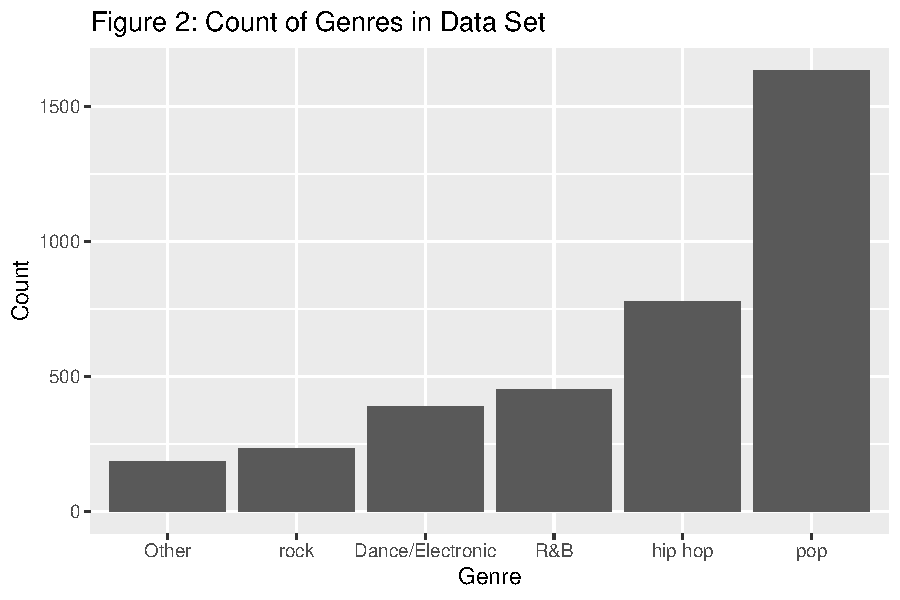
\includegraphics{project_part1_files/figure-latex/top-genres-plot-1.pdf}

This plot shows the popularity/count of each of the genres. In our data,
a song my be included in more than one genre. For example, a song my be
included considered both rock and pop. Therefore, in this plot, if a
song is included in more than one category, let's say, for example, rock
and pop, then this song would be included in count of both the rock and
pop. These genres can help us visualize the proportion of genres of
music that have been considered popular in the past two decades.

\begin{Shaded}
\begin{Highlighting}[]
\FunctionTok{ggplot}\NormalTok{(songs\_filtered, }\FunctionTok{aes}\NormalTok{(}\AttributeTok{x =}\NormalTok{ popularity)) }\SpecialCharTok{+}
  \FunctionTok{geom\_histogram}\NormalTok{(}\AttributeTok{bins =} \DecValTok{30}\NormalTok{, }\AttributeTok{color=}\StringTok{"white"}\NormalTok{, }\AttributeTok{alpha =} \FloatTok{0.6}\NormalTok{, }\FunctionTok{aes}\NormalTok{(}\AttributeTok{y =}\NormalTok{ ..density..)) }\SpecialCharTok{+} 
  \FunctionTok{geom\_density}\NormalTok{(}\AttributeTok{alpha =} \FloatTok{0.6}\NormalTok{, }\AttributeTok{linewidth =} \FloatTok{1.2}\NormalTok{) }\SpecialCharTok{+}
  \FunctionTok{labs}\NormalTok{(}\AttributeTok{title =} \StringTok{" Popularity Distribution with Density Curve"}\NormalTok{,  }
       \AttributeTok{x =} \StringTok{"Popularity"}\NormalTok{,}
       \AttributeTok{y =} \StringTok{"Density"}\NormalTok{) }\SpecialCharTok{+}
  \FunctionTok{theme\_minimal}\NormalTok{() }\SpecialCharTok{+} 
  \FunctionTok{theme}\NormalTok{(}\AttributeTok{plot.title =} \FunctionTok{element\_text}\NormalTok{(}\AttributeTok{size =} \DecValTok{16}\NormalTok{),}
        \AttributeTok{axis.title =} \FunctionTok{element\_text}\NormalTok{(}\AttributeTok{size =} \DecValTok{14}\NormalTok{)) }\SpecialCharTok{+}
  \FunctionTok{geom\_vline}\NormalTok{(}\AttributeTok{xintercept =} \FunctionTok{mean}\NormalTok{(song\_data}\SpecialCharTok{$}\NormalTok{popularity), }
             \AttributeTok{color =} \StringTok{"red"}\NormalTok{, }\AttributeTok{linetype =} \StringTok{"dashed"}\NormalTok{,}
             \AttributeTok{size =} \DecValTok{1}\NormalTok{,}
             \AttributeTok{mapping =} \FunctionTok{aes}\NormalTok{(}\AttributeTok{xintercept =} \FunctionTok{mean}\NormalTok{(popularity)))}
\end{Highlighting}
\end{Shaded}

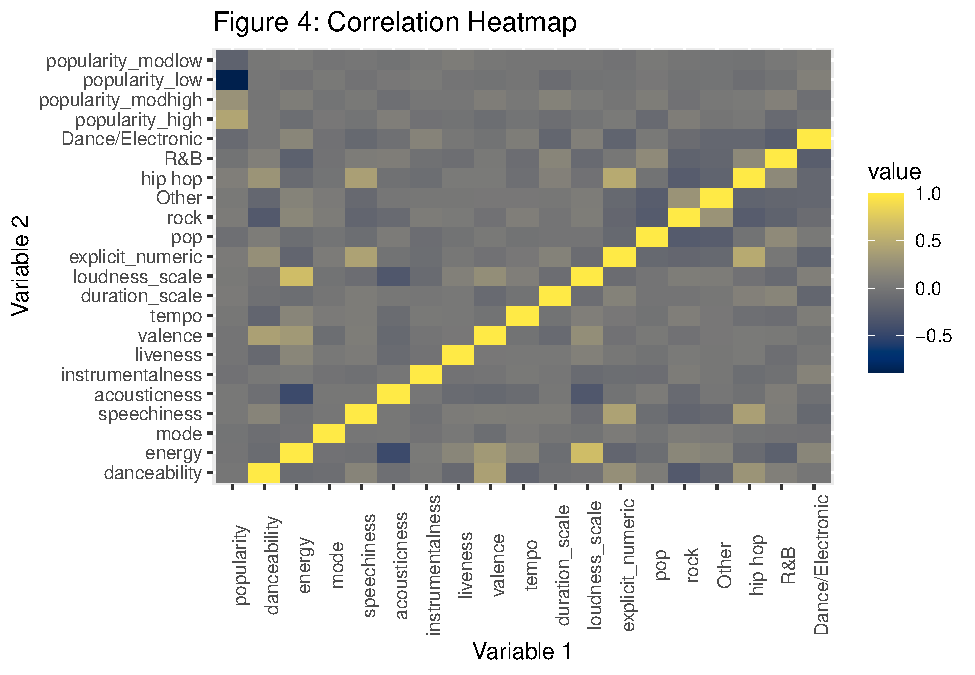
\includegraphics{project_part1_files/figure-latex/unnamed-chunk-5-1.pdf}

This plot shows the distrubution of (scaled) popularity for the songs in
our dataset. The red dash represents the overall mean of the
distribution, 65. The popularity values within our distribution are
centered mostly around 50 through 75.

\begin{Shaded}
\begin{Highlighting}[]
\FunctionTok{ggplot}\NormalTok{(songs\_filtered, }\FunctionTok{aes}\NormalTok{(}\AttributeTok{x =}\NormalTok{ valence, }\AttributeTok{y =}\NormalTok{ popularity)) }\SpecialCharTok{+}
  \FunctionTok{geom\_point}\NormalTok{(}\AttributeTok{alpha =} \FloatTok{0.4}\NormalTok{, }\AttributeTok{color =} \StringTok{"red"}\NormalTok{) }\SpecialCharTok{+} 
  \FunctionTok{geom\_smooth}\NormalTok{(}\AttributeTok{method =} \StringTok{"lm"}\NormalTok{, }\AttributeTok{color =} \StringTok{"blue"}\NormalTok{) }\SpecialCharTok{+}
  \FunctionTok{labs}\NormalTok{(}
    \AttributeTok{title =} \StringTok{"Popularity vs Valence"}\NormalTok{,}
    \AttributeTok{x =} \StringTok{"Valence"}\NormalTok{,}
    \AttributeTok{y =} \StringTok{"Popularity"}
\NormalTok{  ) }\SpecialCharTok{+}
  \FunctionTok{theme\_bw}\NormalTok{()}
\end{Highlighting}
\end{Shaded}

\begin{verbatim}
## `geom_smooth()` using formula = 'y ~ x'
\end{verbatim}

\includegraphics{project_part1_files/figure-latex/unnamed-chunk-6-1.pdf}

This plots shows popularility of song as a function of valence (which
measures the ``postiveness'' conveyed by the track.) From observation of
the plot, there doesn't appear to be a strong linear trend in one
direction or another (although the linear fit is slightly negative in
the plot).

\begin{Shaded}
\begin{Highlighting}[]
\FunctionTok{ggplot}\NormalTok{(songs\_filtered, }\FunctionTok{aes}\NormalTok{(}\AttributeTok{x =}\NormalTok{ danceability, }\AttributeTok{y =}\NormalTok{ popularity)) }\SpecialCharTok{+}
  \FunctionTok{geom\_point}\NormalTok{(}\AttributeTok{alpha =} \FloatTok{0.4}\NormalTok{, }\AttributeTok{color =} \StringTok{"red"}\NormalTok{) }\SpecialCharTok{+} 
  \FunctionTok{geom\_smooth}\NormalTok{(}\AttributeTok{method =} \StringTok{"lm"}\NormalTok{, }\AttributeTok{color =} \StringTok{"blue"}\NormalTok{) }\SpecialCharTok{+}
  \FunctionTok{labs}\NormalTok{(}
    \AttributeTok{title =} \StringTok{"Popularity vs Dancability"}\NormalTok{,}
    \AttributeTok{x =} \StringTok{"Danceability"}\NormalTok{,}
    \AttributeTok{y =} \StringTok{"Popularity"}
\NormalTok{  ) }\SpecialCharTok{+}
  \FunctionTok{theme\_bw}\NormalTok{()}
\end{Highlighting}
\end{Shaded}

\begin{verbatim}
## `geom_smooth()` using formula = 'y ~ x'
\end{verbatim}

\includegraphics{project_part1_files/figure-latex/unnamed-chunk-7-1.pdf}

This plots shows popularity of song as a function of dancibility. From
observation of the plot, there doesn't appear to be a strong linear
trend in one direction or another.

\begin{Shaded}
\begin{Highlighting}[]
\FunctionTok{ggplot}\NormalTok{(songs\_filtered, }\FunctionTok{aes}\NormalTok{(}\AttributeTok{x =}\NormalTok{ duration\_ms}\SpecialCharTok{/}\DecValTok{1000}\SpecialCharTok{/}\DecValTok{60}\NormalTok{)) }\SpecialCharTok{+}
  \FunctionTok{geom\_histogram}\NormalTok{(}\AttributeTok{bins =} \DecValTok{30}\NormalTok{, }\AttributeTok{color=}\StringTok{"white"}\NormalTok{, }\AttributeTok{alpha =} \FloatTok{0.6}\NormalTok{, }\FunctionTok{aes}\NormalTok{(}\AttributeTok{y =}\NormalTok{ ..density..)) }\SpecialCharTok{+} 
  \FunctionTok{geom\_density}\NormalTok{(}\AttributeTok{alpha =} \FloatTok{0.6}\NormalTok{, }\AttributeTok{linewidth =} \FloatTok{1.2}\NormalTok{) }\SpecialCharTok{+}
  \FunctionTok{labs}\NormalTok{(}\AttributeTok{title =} \StringTok{"Songs Duration Distribution with Density Curve"}\NormalTok{,  }
       \AttributeTok{x =} \StringTok{"Duration (Minutes)"}\NormalTok{,}
       \AttributeTok{y =} \StringTok{"Density"}\NormalTok{) }\SpecialCharTok{+}
  \FunctionTok{theme\_minimal}\NormalTok{() }\SpecialCharTok{+} 
  \FunctionTok{theme}\NormalTok{(}\AttributeTok{plot.title =} \FunctionTok{element\_text}\NormalTok{(}\AttributeTok{size =} \DecValTok{16}\NormalTok{),}
        \AttributeTok{axis.title =} \FunctionTok{element\_text}\NormalTok{(}\AttributeTok{size =} \DecValTok{14}\NormalTok{)) }\SpecialCharTok{+}
  \FunctionTok{geom\_vline}\NormalTok{(}\AttributeTok{xintercept =} \FunctionTok{mean}\NormalTok{(song\_data}\SpecialCharTok{$}\NormalTok{duration\_ms}\SpecialCharTok{/}\DecValTok{1000}\SpecialCharTok{/}\DecValTok{60}\NormalTok{), }
             \AttributeTok{color =} \StringTok{"red"}\NormalTok{, }\AttributeTok{linetype =} \StringTok{"dashed"}\NormalTok{,}
             \AttributeTok{size =} \DecValTok{1}\NormalTok{,}
             \AttributeTok{mapping =} \FunctionTok{aes}\NormalTok{(}\AttributeTok{xintercept =} \FunctionTok{mean}\NormalTok{(duration\_ms}\SpecialCharTok{/}\DecValTok{1000}\SpecialCharTok{/}\DecValTok{60}\NormalTok{)))}
\end{Highlighting}
\end{Shaded}

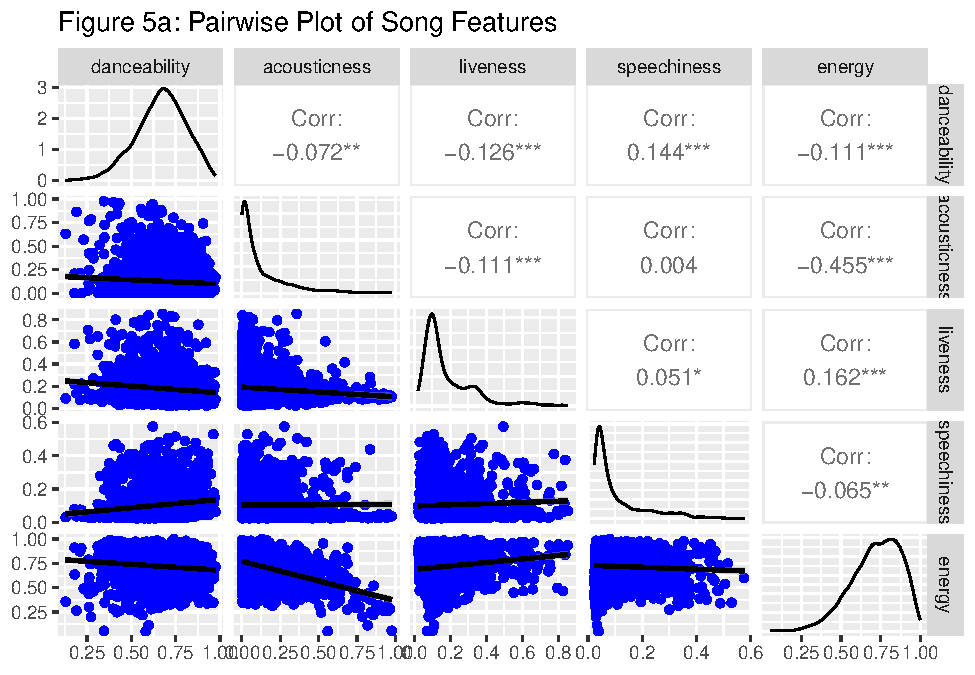
\includegraphics{project_part1_files/figure-latex/unnamed-chunk-8-1.pdf}\\
This plot shows the distribution of song duration in minutes for the
songs in our dataset. As can be seen above, the songs in our dataset
have a mean duration of just under 4 minutes. This can be used to
analyzed to see if longer or shorter songs tend to cause more
popularity.

\begin{Shaded}
\begin{Highlighting}[]
\CommentTok{\# Create correlation matrix}

\FunctionTok{library}\NormalTok{(viridis)}
\end{Highlighting}
\end{Shaded}

\begin{verbatim}
## Loading required package: viridisLite
\end{verbatim}

\begin{Shaded}
\begin{Highlighting}[]
\NormalTok{cor\_mat }\OtherTok{\textless{}{-}} \FunctionTok{cor}\NormalTok{(songs\_filtered }\SpecialCharTok{\%\textgreater{}\%} 
                \FunctionTok{select\_if}\NormalTok{(is.numeric))}

\CommentTok{\# Use reshape2 to melt the matrix}
\FunctionTok{library}\NormalTok{(reshape2)}
\end{Highlighting}
\end{Shaded}

\begin{verbatim}
## 
## Attaching package: 'reshape2'
\end{verbatim}

\begin{verbatim}
## The following object is masked from 'package:tidyr':
## 
##     smiths
\end{verbatim}

\begin{Shaded}
\begin{Highlighting}[]
\NormalTok{melted\_cor }\OtherTok{\textless{}{-}} \FunctionTok{melt}\NormalTok{(cor\_mat) }

\CommentTok{\# Plot heatmap}
\FunctionTok{ggplot}\NormalTok{(}\AttributeTok{data =}\NormalTok{ melted\_cor, }\FunctionTok{aes}\NormalTok{(}\AttributeTok{x=}\NormalTok{Var1, }\AttributeTok{y=}\NormalTok{Var2, }\AttributeTok{fill=}\NormalTok{value)) }\SpecialCharTok{+} 
  \FunctionTok{geom\_tile}\NormalTok{() }\SpecialCharTok{+}
  \FunctionTok{scale\_fill\_viridis}\NormalTok{() }\SpecialCharTok{+}
  \FunctionTok{theme}\NormalTok{(}\AttributeTok{axis.text.x =} \FunctionTok{element\_text}\NormalTok{(}\AttributeTok{angle =} \DecValTok{90}\NormalTok{)) }\SpecialCharTok{+}
  \FunctionTok{labs}\NormalTok{(}
    \AttributeTok{title=}\StringTok{"Correlation Heatmap"}\NormalTok{,}
    \AttributeTok{x =} \StringTok{"Variable 1"}\NormalTok{,}
    \AttributeTok{y =} \StringTok{"Variable 2"}
\NormalTok{  ) }
\end{Highlighting}
\end{Shaded}

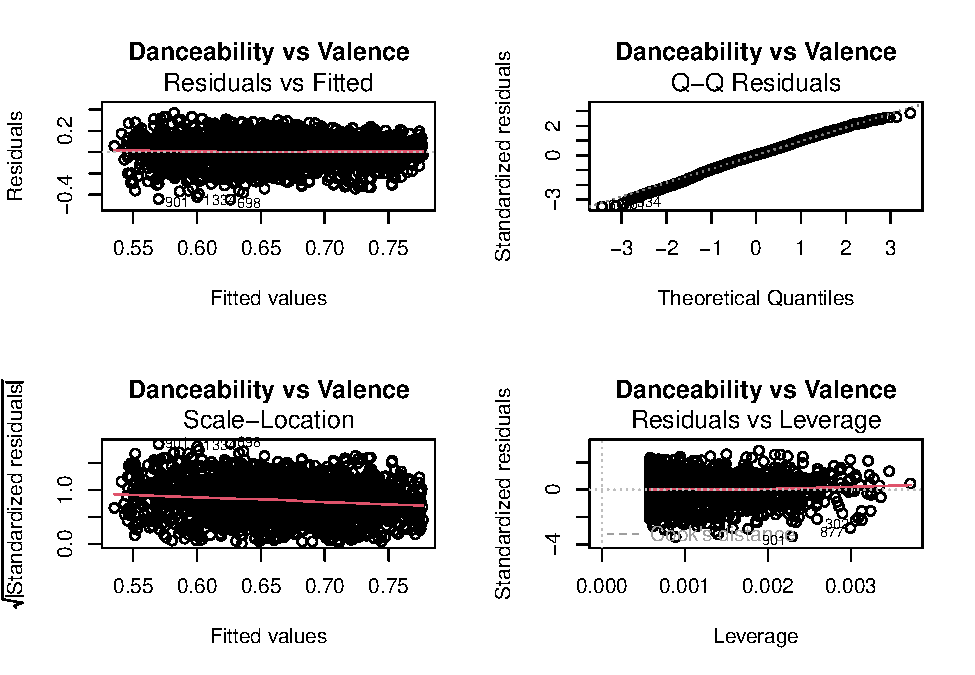
\includegraphics{project_part1_files/figure-latex/unnamed-chunk-9-1.pdf}

This plot shows the correlation between each variable in our dataset (as
a matrix heatmap). The darker colors show negative correlation while the
warmer colors (more yellow) show more positive correlation. For example,
from the plot above we can see that acoustiness and energy have a
negative correlation, while loudness and energy have a positive
correlation (both of which are intuitive). Another interesting
observation is that the release year is negatively correlated with
duration, which indicates that songs have been getting shorter in recent
times.

\begin{Shaded}
\begin{Highlighting}[]
\NormalTok{m2 }\OtherTok{\textless{}{-}} \FunctionTok{lm}\NormalTok{(}\AttributeTok{formula =}\NormalTok{ popularity }\SpecialCharTok{\textasciitilde{}}\NormalTok{ danceability }\SpecialCharTok{+} 
\NormalTok{          energy }\SpecialCharTok{+}\NormalTok{ loudness }\SpecialCharTok{+}\NormalTok{ acousticness }\SpecialCharTok{+}\NormalTok{ mode }\SpecialCharTok{+}  
\NormalTok{          speechiness }\SpecialCharTok{+}\NormalTok{ liveness  }\SpecialCharTok{+}\NormalTok{ valence }\SpecialCharTok{+}\NormalTok{ tempo }\SpecialCharTok{+}
\NormalTok{          duration\_ms, }\AttributeTok{data =}\NormalTok{ songs\_filtered)}

\FunctionTok{par}\NormalTok{(}\AttributeTok{mfrow=}\FunctionTok{c}\NormalTok{(}\DecValTok{2}\NormalTok{,}\DecValTok{2}\NormalTok{)) }
\FunctionTok{plot}\NormalTok{(m2)}
\end{Highlighting}
\end{Shaded}

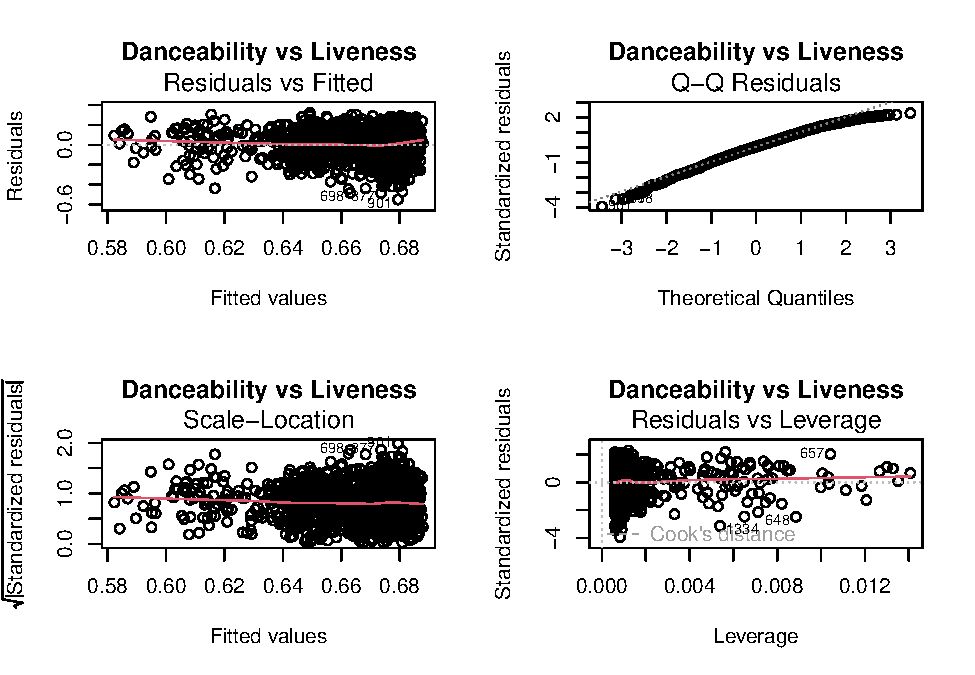
\includegraphics{project_part1_files/figure-latex/unnamed-chunk-10-1.pdf}\\
In the Residuals vs Fitted plot, we can see that the variance does not
increase or decrease in one direction of the other, however there does
appear to be more variance in the middle ranges. Therefore, a
transformation of the explanatory variable may be necessary. As for the
assumption of linearity, this plot appears to be fairly linear.\\
In the Normal Q-Q Plot, we see some deviation from normality, especially
at the tails. This result indicates that our data has heavy tails or
potential outliers. We may need to consider transformations of the
response or explanatory variable.\\
The Scale-Location plot generally shows more varibility in the residuals
in the middle values, which may indicate a violation of our assumption
of constant variance of errors. Therefore, we may need to consider a
transformation of the explanatory variable.\\
Finally, the Residuals vs Leverage plot, which helps us identify
influential/disproportionate observations in our model, shows more
variance of the residuals on the left. This suggests that observations
with lower leverage show more variability. Furthermore, there aren't
many observation on the right side of our plot, indicating there few
very points that are (individually) highly influential on our regression
model. These observations merit more analysis.\\

\hypertarget{insights}{%
\subsection{Insights}\label{insights}}

The data was somewhat surprising in terms of how spread out it was. The
plots did not show clear linear associations and there were a lot of
residuals. However, the sampling itself went well - with 2,000 different
data points spanning popular songs from the past two decades, we likely
got a fair representation of worldwide music popularity trends in that
timeframe.

A few caveats around how representative the sample is: the data does not
include songs from the most recent 5 years, so very current trends are
missing. Additionally, we don't know exactly how the ``popularity''
statistic was measured. There could also be shifting trends over time as
what is popular changes year to year. But with 2,000 songs across
multiple decades, many of those temporal effects should be smoothed out.

Overall, while surprising in some regards, the wide sampling over an
extended retrospective time period should provide a reasonable snapshot
of historically popular music. Factors like recency and the vagueness of
the popularity metric likely impact the data, but not enough to
undermine how representative the 2000 song sample is of the last 20
years. The key time-related factor is that very current trends are
omitted given the data ends 5 years ago.

\end{document}
